\section{Première formulation robuste}
\subsection{Modèle}
%Afin de prendre en compte les erreurs sur les facteurs d'amplification $x_i$, nous utilisons les valeurs maximales des variations possibles de $\hat{D(\theta)}$ sur un intervalle.\\
%\begin{equation}
%|\hat{D(\theta)}|  =  |\sum_{i=1}^{n} x_i(1+\xi_i)d_i(\theta)| \leq  |\sum_{i=1}^{n} x_i d_i(\theta)| + |\sum_{i=1}^{n} x_i \xi_i d_i(\theta)|  \leq  |D(\theta)| + \sum_{i=1}^{n} |\tau x_i d_i(\theta)\frac{h}{2}| 
%\end{equation}
%En imposant $|D(\theta)| + \sum_{i=1}^{n} | \tau x_i d_i(\theta)\frac{h}{2}|\leq \epsilon $ on est sur que $|\hat{D(\theta)}|\leq \epsilon$. On traduit les contraintes sur $\mathcal{P}$ comme $|D(\theta)-1| + \sum_{i=1}^{n} |\tau x_i d_i(\theta)\frac{h}{2}|\leq \epsilon $ de la même manière. 
%Pour notre problème échantillonné et linéaire, il nous faut donc introduire $n$ variables $v_i$ (associées à chaque $\theta$ échantillonné) correspondant aux valeurs absolues des $\tau d_i(\theta)\frac{h}{2}$. On a alors le modèle : 
%\begin{align}
%|D(\theta)| + \sum_{i=1}^{n} v_i & \leq  \epsilon & \forall i \in \mathcal{S} \\
%|D(\theta)-1| + \sum_{i=1}^{n}v_i & \leq  \epsilon & \forall i \in \mathcal{P} \\
%\tau x_i d_i(\theta)\frac{h}{2} & \leq  v_i \\
%-\tau x_i d_i(\theta)\frac{h}{2} & \leq  v_i 
%\end{align}

Afin de prendre en compte les erreurs sur les facteurs d'amplification $x_i$, nous utilisons les valeurs maximales des variations possibles de $\hat{D(\theta)}$ sur un intervalle.\\
\begin{equation}
|\hat{D(\theta)}|  =  |\sum_{i=1}^{n} x_i(1+\xi_i)d_i(\theta)| \leq  |\sum_{i=1}^{n} x_i d_i(\theta)| + |\sum_{i=1}^{n} x_i \xi_i d_i(\theta)|  \leq  |D(\theta)| + \sum_{i=1}^{n} |\tau x_i d_i(\theta)| 
\end{equation}
En imposant $|D(\theta)| + \sum_{i=1}^{n} | \tau x_i d_i(\theta)\leq \epsilon $ on est sur que $|\hat{D(\theta)}|\leq \epsilon$. On traduit de la même manière les contraintes sur $\mathcal{P}$ comme $|D(\theta)-1| + \sum_{i=1}^{n} |\tau x_i d_i(\theta)|\leq \epsilon $ . 
Pour notre problème échantillonné et linéaire, il nous faut donc introduire $n$ variables $v_i$ (associées à chaque $\theta$ échantillonné) correspondant aux valeurs absolues des $\tau d_i(\theta)$. On a alors le modèle : 
\begin{align}
|D(\theta)| + \sum_{i=1}^{n} v_i & \leq  \epsilon & \forall i \in \mathcal{S} \\
|D(\theta)-1| + \sum_{i=1}^{n}v_i & \leq  \epsilon & \forall i \in \mathcal{P} \\
\tau x_i d_i(\theta) & \leq  v_i \\
-\tau x_i d_i(\theta) & \leq  v_i 
\end{align}

\subsection{Analyse des résultats}
Les figures \ref{fig:D-ModRobust1}, \ref{fig:D-ModRobust1-test3RobTau001} et \ref{fig:D-ModRobust1-test3RobTau01} montrent les résultats obtenus pour différentes valeurs de $\tau$ (dans le modèle ainsi que dans les perturbations). Ici les $x$ sont conçus pour mieux résister en cas de perturbations. Un récapitulatif des résultats pour les différents modèle est donné à la table \ref{table:Recap}. Notons que ces modèles sont bien plus performant que le modèle de base. En effet le $\epsilon$ augmente très peu $2\%$ dans le modèle de base à $2.8\%$ ou $3.3\%$ dans le modèle robuste; tandis que la robustesse s'améliore nettement.\\
\begin{itemize}
\item Dans le cas $\tau = 0.001$, on constate une augmentation du $\epsilon$ par rapport au modèle de base. Les erreurs pour les $x_i$ perturbés sont cependant bien moindre. On constate également que les erreurs pour le modèle $x_i$ perturbés avec une perturbation de l'ordre de $\tau=0.001$ ou de $\tau = 0.01$ sont moindre que dans le modèle avec $\tau=0.01$. Mais malgré que les erreurs soient moindre que dans le modèle $\tau = 0.01$ même dans le cas où les perturbations sont de l'ordre de $\tau =0.01$, on  observe des dépassements pour certaines réalisation des $\xi_i$ si on applique les perturbations de $\tau=0.01$. On constate que l'ordre de grandeur des $x_i$ non-nuls est inférieur à celui du modèle de base ce qui confirme notre intuition comme quoi le modèle robuste a tendance à fournir des $x_i$ plus petits.\\ 
 \item Dans le cas $\tau = 0.01$, on constate toujours une augmentation du $\epsilon$ par rapport au modèle de base et au modèle où $\tau = 0.001$. Les erreurs pour les $x_i$ perturbés sont plus grande que dans le modèle $\tau=0.001$ pour des perturbations de l'ordre de $\tau = 0.001$ et $\tau=0.01$, mais le modèle ne présente jamais de dépassement. On constate que l'ordre de grandeur des $x_i$ non-nuls est inférieur à celui du modèle $\tau=0.001$, ce qui confirme encore notre intuition.
\end{itemize}

\begin{figure}[h!]
  \centering
  \begin{subfigure}[b]{0.45\textwidth}
  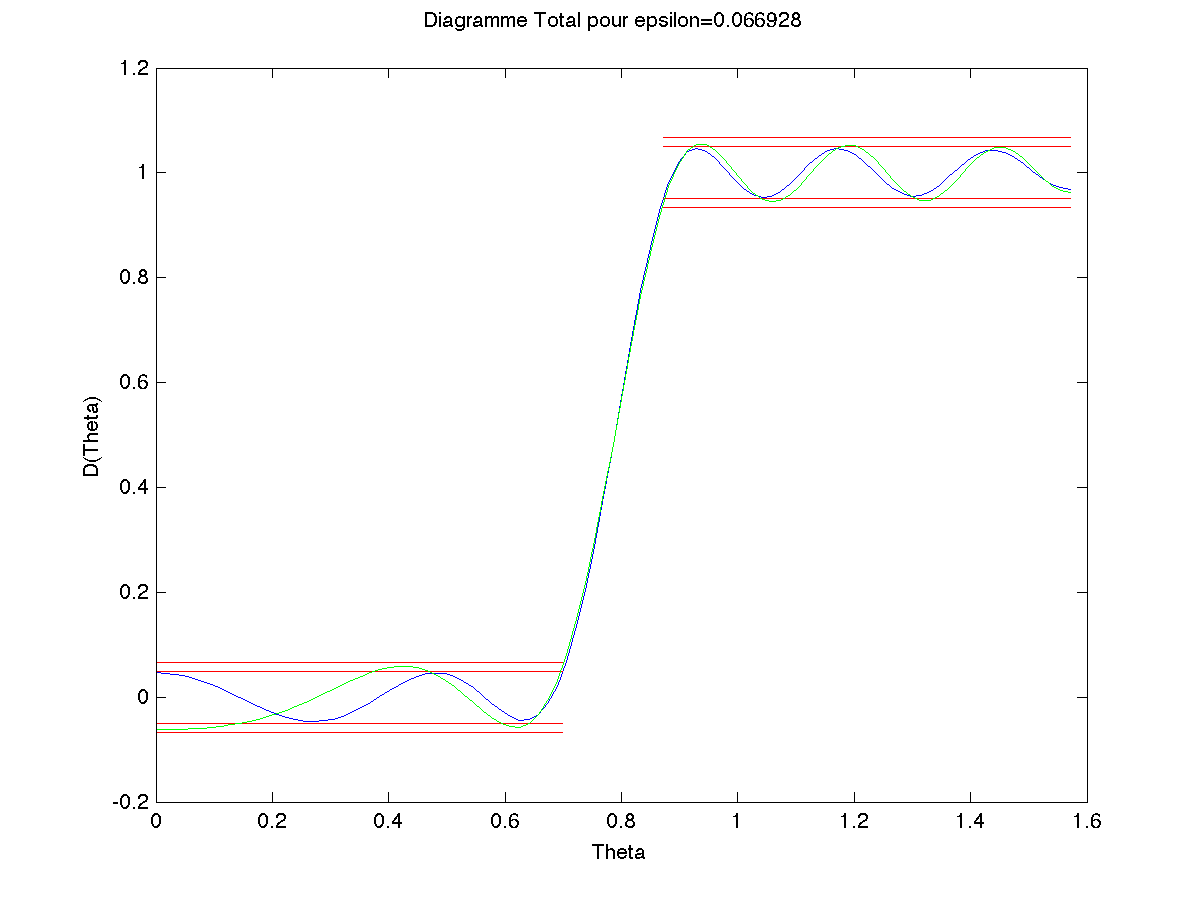
\includegraphics[width=\textwidth]{D-ModRobust1.png}
  \caption{$D(\theta)$ pour le modèle $\tau = 0.01$ (en vert) et $\tau = 0.001$ (en bleu) et $x$ non-perturbé.}
  \label{fig:D-ModRobust1}
  \end{subfigure}
  ~ 
 \begin{subfigure}[b]{0.45\textwidth}
  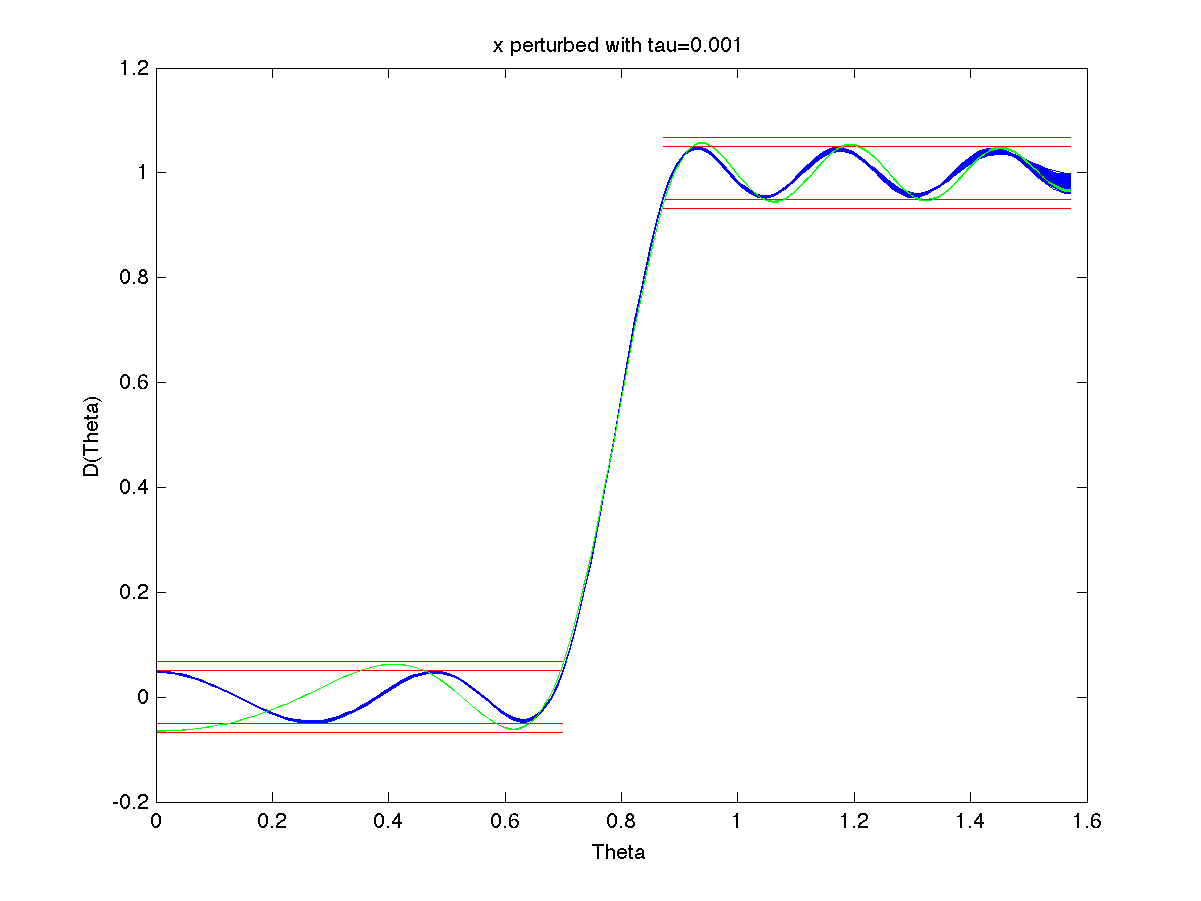
\includegraphics[width=\textwidth]{D-ModRobust1-test3Rob001.png}
  \caption{$D(\theta)$ pour une perturbation de $\tau = 0.001$ sur les $x$ (en vert pour un modèle de $\tau=0.01$ en bleu pour $\tau=0.001$).}
  \label{fig:D-ModRobust1-test3RobTau001}
  \end{subfigure}
  \begin{subfigure}[b]{0.45\textwidth}
  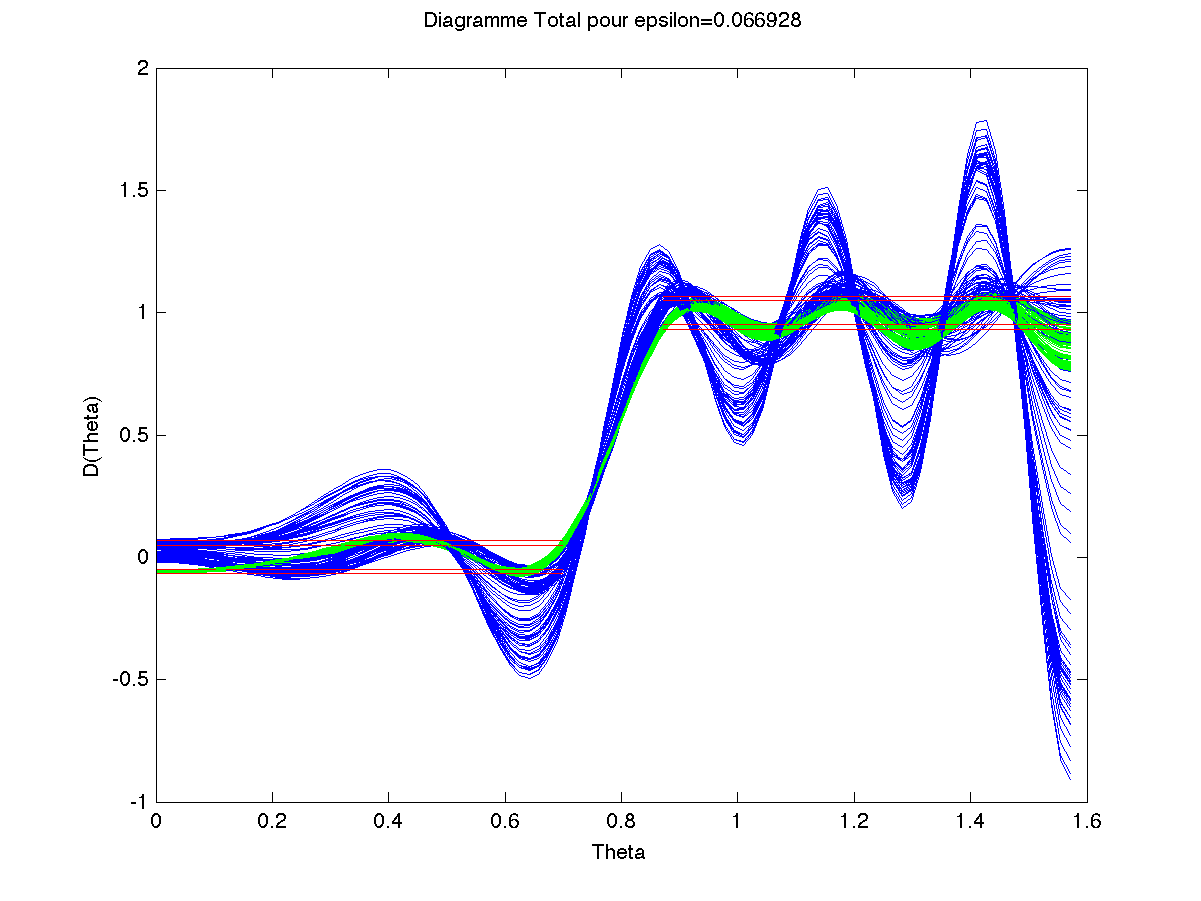
\includegraphics[width=\textwidth]{D-ModRobust1-test3Rob01.png}
  \caption{$D(\theta)$ pour une perturbation de $\tau = 0.01$ sur les $x$ (en vert pour un modèle de $\tau=0.01$ en bleu pour $\tau=0.001$).}
  \label{fig:D-ModRobust1-test3RobTau01}
  \end{subfigure}
  \caption{Les deux derniers graphes sont donnés pour une centaine de réalisations des $\xi_i$.}
  \end{figure}

\begin{table}
\centering
\begin{tabular}{c|c|c|ccc}
 & & &  &\textbf{Erreurs pour : } &\\
 & $\epsilon$ & $\mathcal{O}( x_i)$ ($x_i\neq0$ &$x_i$ & $x_i$ pert. ($\tau=0.001$) & $x_i$ pert. ($\tau=0.01$) \\
 \hline
Modèle de base & $2\%$ & $10^3$ &0.0185 & 5.3977 & 47.9054 \\
Modèle robuste 1 ($\tau=0.001$) & $5.07 \%$ & $10^0$& 0.0396 & 0.0396  & 0.0440 \\
Modèle robuste 1 ($\tau=0.01$)  & $6.80 \%$ &$10^{-1}$ &0.0508 & 0.0508 & 0.0510 \\
\end{tabular}
\caption{Récapitulatif des résultats des erreurs et de la borne maximal $\epsilon$ obtenus pour les différents modèles et les différents types de perturbations.}
\label{table:Recap}
\end{table}